\chapter{Experiments: Lattices}
\label{ch:regular-tilings}

% (TODO): Overall: standard deviations.

% (TODO): Remember to always specify specifics of experiment setups for all
% experiments

% (TODO): t!
\begin{figure*}[t]
  \centering
  \begin{subfigure}{.32\textwidth}
    \centering
    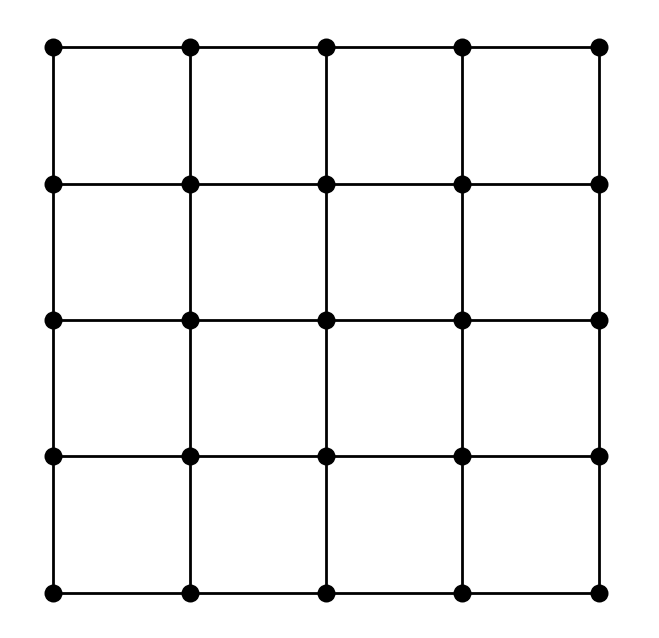
\includegraphics[width=1.0\linewidth]{figures/square.png}
    \label{fig:rt-square}
  \end{subfigure}
  \begin{subfigure}{.32\textwidth}
    \centering
    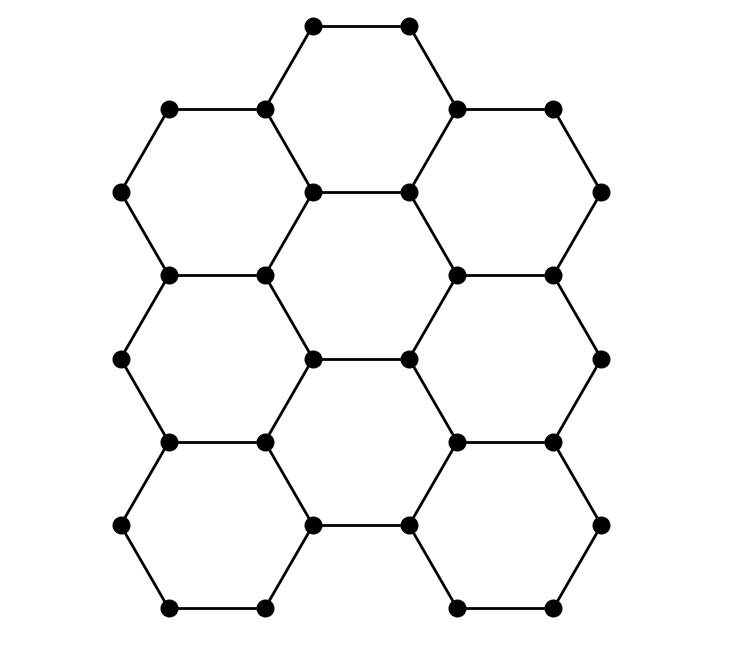
\includegraphics[width=1.0\linewidth]{figures/hex.png}
    \label{fig:rt-hex}
  \end{subfigure}
  \begin{subfigure}{.32\textwidth}
    \centering
    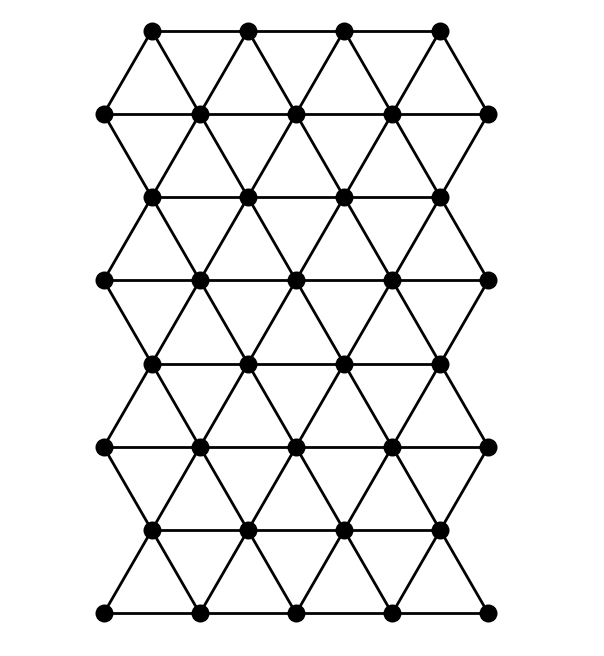
\includegraphics[width=1.0\linewidth]{figures/triangular.png}
    \label{fig:rt-tri}
  \end{subfigure}
  \caption{
    Types of lattices investigated for their quality as reservoir
topologies. Investigated tilings include square (a), hexagonal (b), and
triangular (c).
  }
  \label{fig:regular-tilings}
\end{figure*}

Lattice models are common in computational physics
\cite{lavis_equilibrium_2015}. Understanding important models of computational
physics in reservoir contexts is thus crucial to advance physical RC
methodology. For example, the Ising model with dipole moments of atomic spins
\cite{jensen_computation_2018}, spin-torque oscillator arrays
\cite{tsunegi_physical_2019}, and the Ginzburg-Landau equation
\cite{opala_neuromorphic_2019}, describe systems that are employed on a
two-dimensional lattice, and have been used in reservoir settings. In this
chapter, we therefore investigate lattice networks as more realistic models of
physical reservoirs.

We explore the properties that lattice graphs exhibit as reservoirs by
structuring internal nodes in this manner. Lattice graphs may be embedded in
Euclidean space to form regular tilings, of which there three in two-dimensional
space: square, hexagonal and triangular, which are all depicted in Figure
\ref{fig:regular-tilings}. Other, more complicated tiling schemes
exist. Semiregular, often called uniform, tilings are created using two or more
faces. However, complicated grids are left outside the scope of this thesis, as
our primary focus is the fundamental applicability of lattice layouts, not
comparing the performance between them.

Reservoirs are created by replacing the reservoirs of ESN models with the
adjacency matrix generated for lattice models. For each experiment,
$\mathbf{W}^{res}$ is then scaled to a spectral radius of 0.9, as this is
equivalent to scaling the coupling, or spacing, between nodes in a physical
system. Beyond this, our reservoir model remains the same as that of the ESN.

\textcolor{red}{
  Perhaps a paragraph summarizing each section.
}

\section{Reservoir Quality of Lattices}
\label{sec:lattice-quality}

\subsection{Synopsis}

First, we evaluate the default quality of lattice reservoirs with the NARMA-10
benchmark. Reservoirs are generated by embedding internal nodes in a metric
space, much like in Figure \ref{fig:regular-tilings}, and connecting neighboring
pairs with an edge of unit length. Nodes along the edges are not connected to
the opposite side of the lattice, making the lattice aperiodic. Lastly, unit
weight of all edges are scaled by the appropriate scalar to allow a spectral
radius of 0.9.

\subsection{Results and Discussion}

% (TODO): t!
\begin{figure}[t]
  \centering
  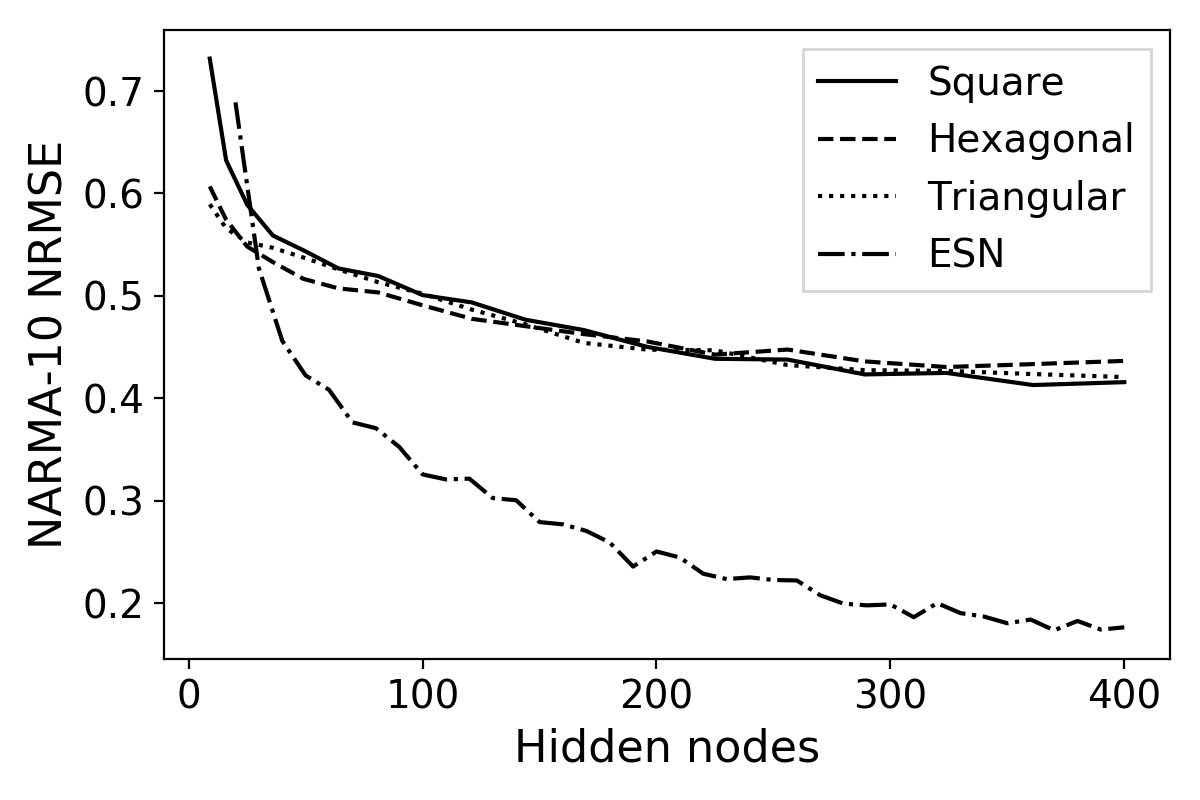
\includegraphics[width=3.5in]{figures/regular-tilings-performance.png}
  \caption{
    NARMA-10 NRMSE of square, hexagonal, and triangular regular tilings as
reservoir topologies.
  }
  \label{fig:rt-performance}
\end{figure}

Figure \ref{fig:rt-performance} shows how reservoir error scales with reservoir
size. We see that restricting reservoir topologies to lattice structures results
in a significant performance penalty. Additionally, little difference is seen
between the three types of tilings.

% (TODO): t!
\begin{figure*}[t]
  \centering
  \begin{subfigure}{.32\textwidth}
    \centering
    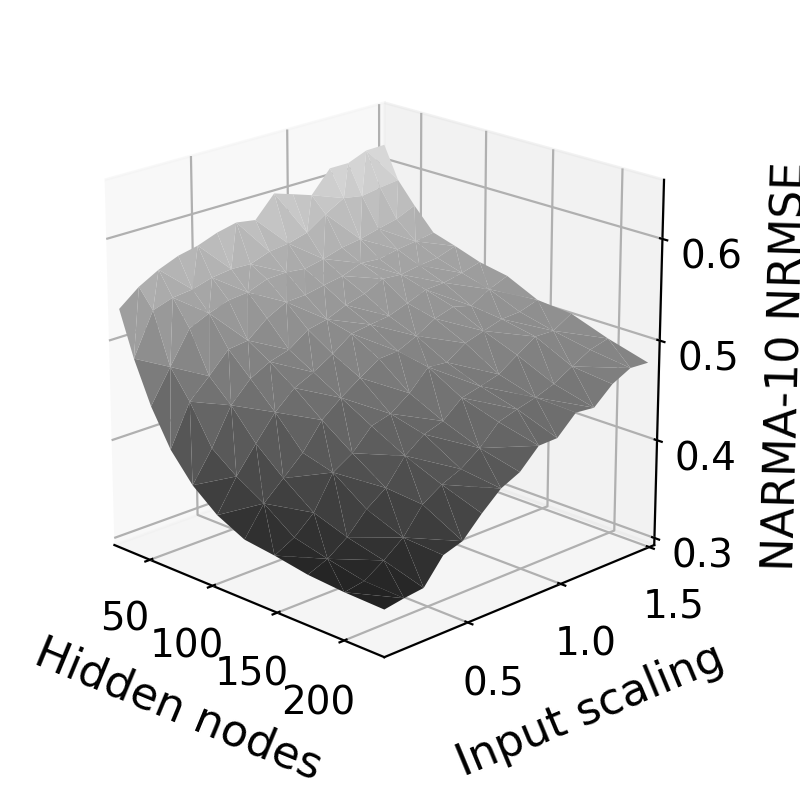
\includegraphics[width=1.0\linewidth]{figures/regular-tilings-performance-is-sq.png}
    \caption{}
    \label{fig:rt-is-square}
  \end{subfigure}
  \begin{subfigure}{.32\textwidth}
    \centering
    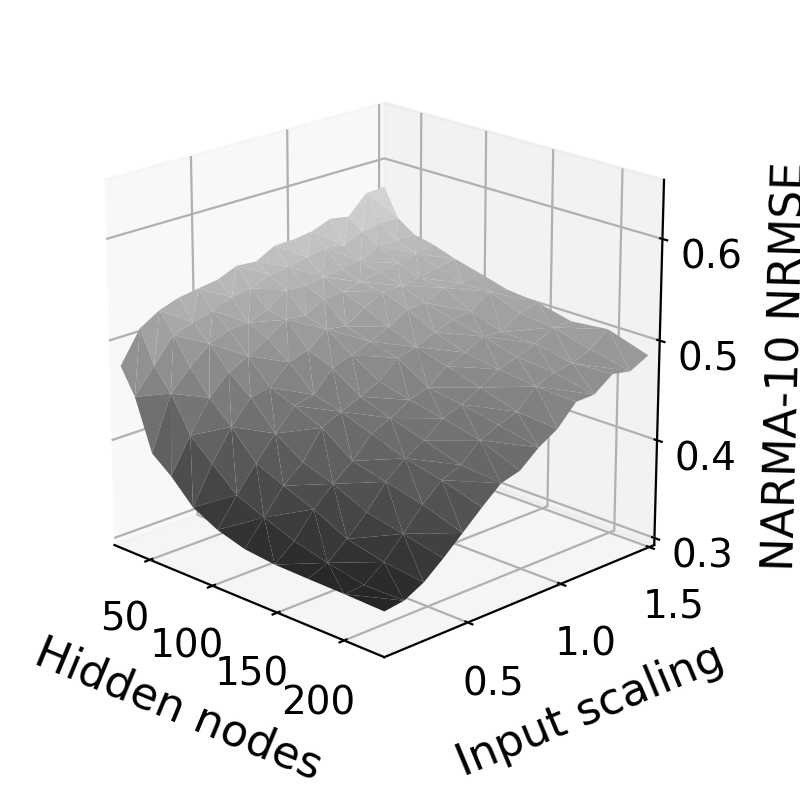
\includegraphics[width=1.0\linewidth]{figures/regular-tilings-performance-is-hex.png}
    \caption{}
    \label{fig:rt-is-hex}
  \end{subfigure}
  \begin{subfigure}{.32\textwidth}
    \centering
    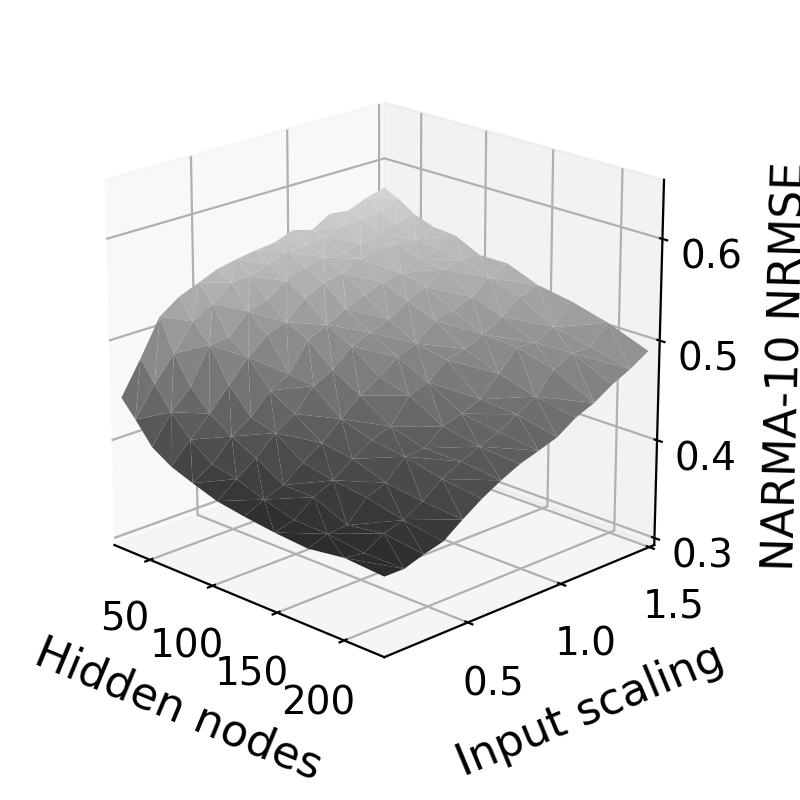
\includegraphics[width=1.0\linewidth]{figures/regular-tilings-performance-is-tri.png}
    \caption{}
    \label{fi:rt-is-tri}
  \end{subfigure}
  \caption{
    Regular tilings investigated for their quality as reservoir topologies, here
as a function of reservoir size and input scaling. Investigated topologies
include square (a), hexagonal (b), and triangular (c) regular tilings.
  }
  \label{fig:rt-performance-is}
\end{figure*}

In Section \ref{sec:dist-func}, it was discovered that reservoirs modeling
random geometric graphs exhibited low memory retention. The symptoms are similar
here: the lattice reservoirs perform worse than a delay line would, and only
perform marginally better with an increasing size. Figure
\ref{fig:rt-performance-is} illustrates the effect of scaling the magnitude of
the input. Again, we see clearly see reservoirs favoring low input scaling
values.

We interpret these results to indicate that the structure imposed by an
undirected lattice shifts the point of criticality described in
\ref{sec:criticality}. When input scaling is lessened such that the required
memory capacity for the benchmark task is reached, the error diminishes rapidly,
and the existing reservoir dynamics work as intended.

Curiously, the NRMSE differs only slightly between the three types of
lattice. It seems that it is the overall lattice structure that is important,
not the specific type of tiling implementing it. We therefore argue that the
different tilings, which in practice dictate the amount of incident edges per
vertex, work mostly as minor tuning parameters. The idea that overall structure
is important is in accordance with our findings in \ref{sec:restore}, concluding
that \textit{how information flows} in the network is vital.

Input scaling decreased the benchmark error of lattice reservoirs, but the best
performing networks of Figure \ref{fig:rt-performance-is} are not quite
comparable to the ESN. For example, square grid reservoirs of size 200 benchmark
a mean NRMSE of around 0.35, while corresponding ESNs average around 0.25.

Overall, it is interesting that undirected lattice reservoirs perform as well as
they do. On the other hand, the distribution of the input weights are drawn from
a uniform distribution in the interval [-0.5, 0.5], letting internal nodes see
varying representations of the input signal. As physical substrates may differ
in the input schemes they offer, the input scheme will be further investigated
in the next section.

To summarize, we have in this section found undirected lattice reservoirs to
provide promising results. A key discovery of Chapter \ref{ch:rgg} is the
importance of a directed flow of information, and whether directedness also
improves lattice models is the topic of the next section.

\section{Lattices with Directed Edges}
\label{sec:lat-dir-edge}

\subsection{Synopsis}

% (TODO): t!
\begin{figure*}[t]
  \centering
  \begin{subfigure}{.40\textwidth}
    \centering
    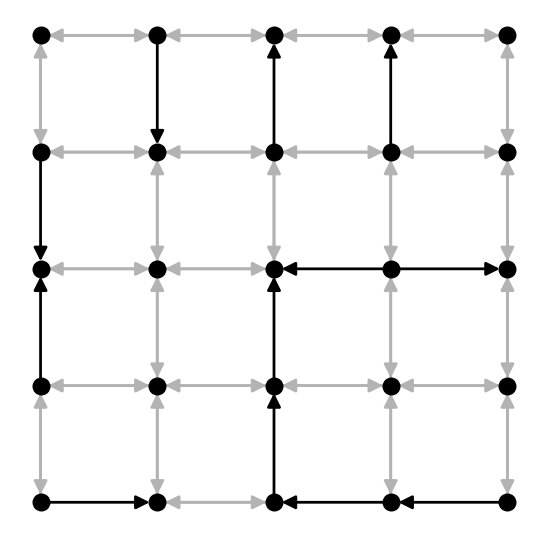
\includegraphics[width=1.0\linewidth]{figures/dir_lattice_025.png}
    \caption{}
    \label{fig:dir-lattice-a}
  \end{subfigure}
  \hspace{25pt}
  \begin{subfigure}{.40\textwidth}
    \centering
    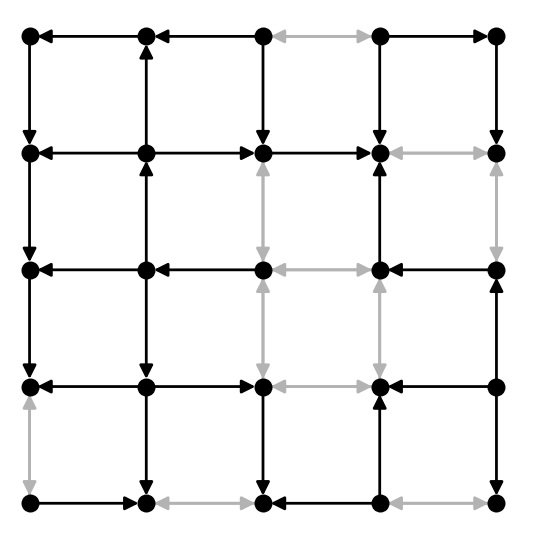
\includegraphics[width=1.0\linewidth]{figures/dir_lattice_075.png}
    \caption{}
    \label{fig:dir-lattice-b}
  \end{subfigure}
  \caption{
    Example square grids where 25\% (a) and 75\% (b) of the undirected edges are
made directed.
  }
  \label{fig:dir-lattice}
\end{figure*}

One of the key discoveries of Chapter \ref{ch:rgg} is that directed edges
improve performance significantly in random geometric graph reservoirs. It is of
interest to repeat this experiment with lattice reservoirs, especially since
information flow is so clearly visible in a lattice structure. We modify the
generated lattice graphs generated in previous sections of this chapter to have
a fraction of directed edges. Figure \ref{fig:dir-lattice} illustrates the
concept for square lattices, where 25\% and 75\% of the edges of the two
lattices, respectively, have been directed. The directed reservoir edges have a
50\% chance of going in either direction.

\subsection{Results and Discussion}

% (TODO): t!
\begin{figure*}[t]
  \centering
  \begin{subfigure}{.32\textwidth}
    \centering
    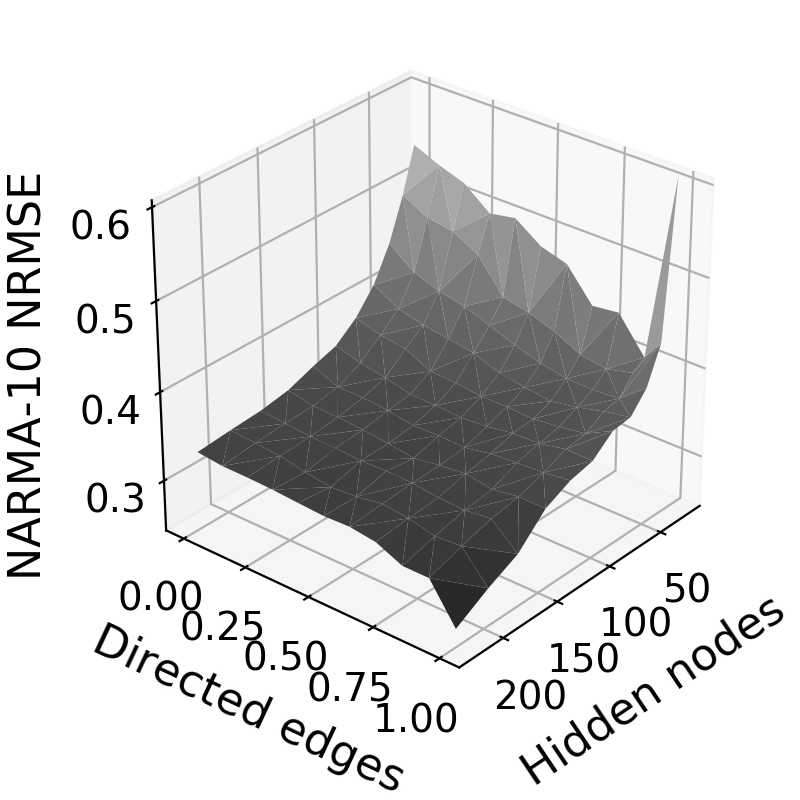
\includegraphics[width=1.0\linewidth]{figures/rt-dir-perf-sq.png}
    \caption{}
    \label{fig:rt-dir-perf-trisurf-sq}
  \end{subfigure}
  \begin{subfigure}{.32\textwidth}
    \centering
    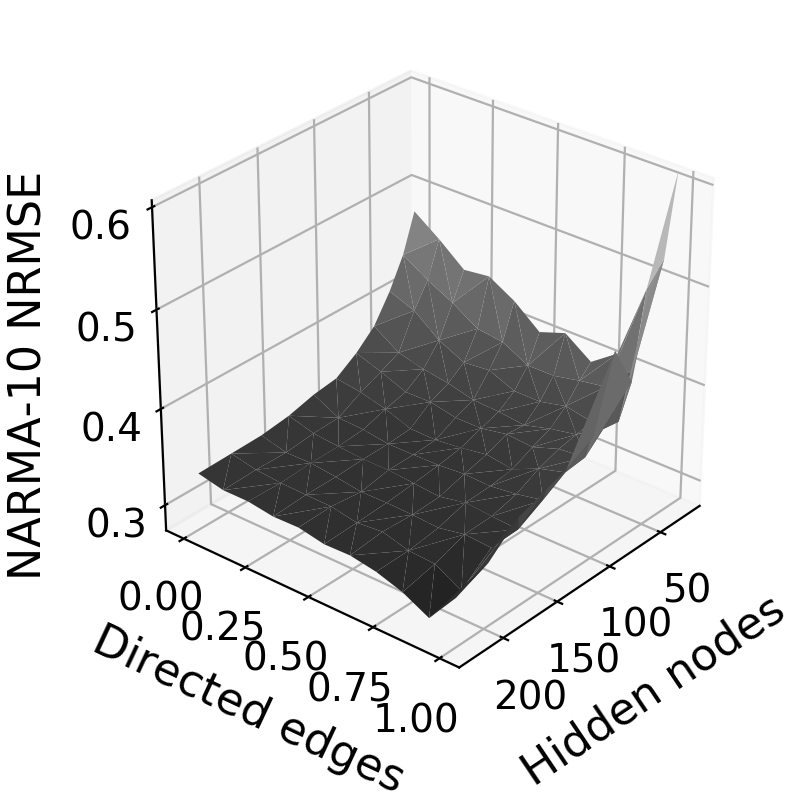
\includegraphics[width=1.0\linewidth]{figures/rt-dir-perf-hex.png}
    \caption{}
    \label{fig:rt-dir-perf-trisurf-hex}
  \end{subfigure}
  \begin{subfigure}{.32\textwidth}
    \centering
    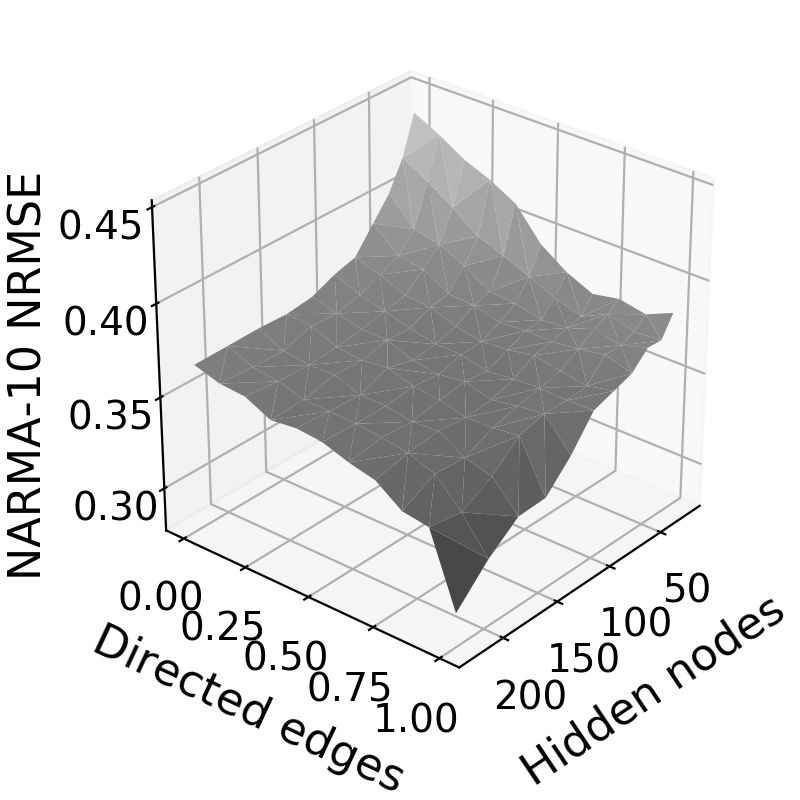
\includegraphics[width=1.0\linewidth]{figures/rt-dir-perf-tri.png}
    \caption{}
    \label{fig:rt-dir-perf-trisurf-tri}
  \end{subfigure}
  \caption{
    Benchmark error as a function of reservoir size and directedness. The
fraction of directed edges determines the amount of edges that are left
bidirectional, explained by Figure \protect\ref{fig:dir-lattice}. Shown are
results for square (a), hexagonal (b) and triangular (c) lattices.
  }
  \label{fig:rt-dir-perf-trisurf}

  \centering
  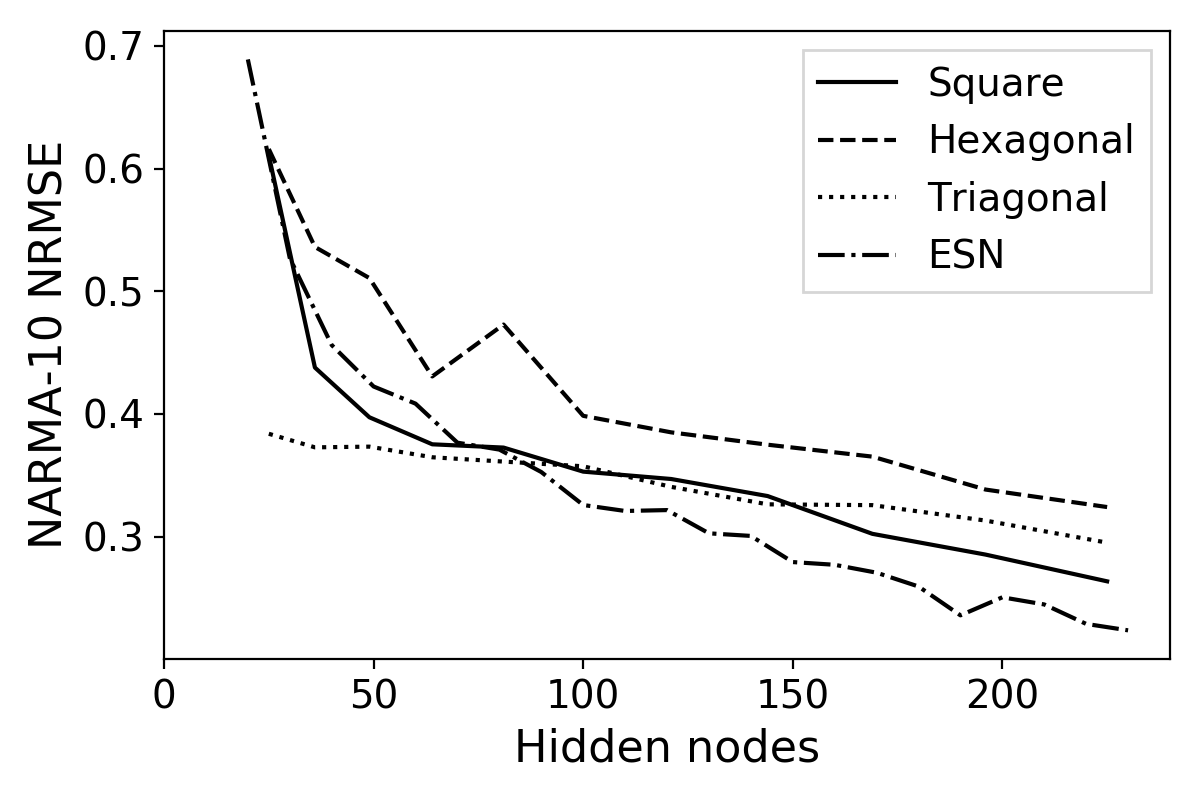
\includegraphics[width=3.5in]{figures/rt-dir-perf.png}
  \caption{
    Benchmark error as a function of size for directed lattice reservoirs. All
reservoirs are fully directed, and the direction of each edge is decided by an
unbiased coin toss.
  }
  \label{fig:rt-dir-perf}
\end{figure*}

Figure \ref{fig:rt-dir-perf-trisurf} presents the results of introducing a
fraction of directed edges to lattice reservoirs. Most reservoirs show reduced
error rates with increasing fractions of directed edges.

A small exception is visible for very small square and hexagonal reservoirs,
where a fully directed reservoir may degrade if the edges align in an
insufficient manner. Nodes in triangular reservoirs have six incident edges, as
opposed to the three and four of square and hexagonal, thus giving a smaller
chance of insufficient reservoirs appearing. Note that this problem disappears
with bigger reservoirs. This compelling result indicates that our method of
generating directed edges guarantees good reservoirs as their sizes increase --
one does not need to ``get lucky'' with directions.

Convincing improvements are exhibited once reservoirs become fully directed and
sufficiently big, which is especially visible at the sudden drops at the closest
points of the surface areas. The drops are only sudden when compared to
reservoirs of a lower fraction of directed edges. We plot the cross section of
the surface areas at full directedness in Figure \ref{fig:rt-dir-perf}, showing
that the error rates keep decreasing with increased reservoir size. This is
again in stark contrast to their undirected counterparts, which in Section
\ref{sec:lattice-quality}, and also previous in Section \ref{sec:restore} only
perform marginally better as reservoir size is increased.

\begin{figure}
  \centering
  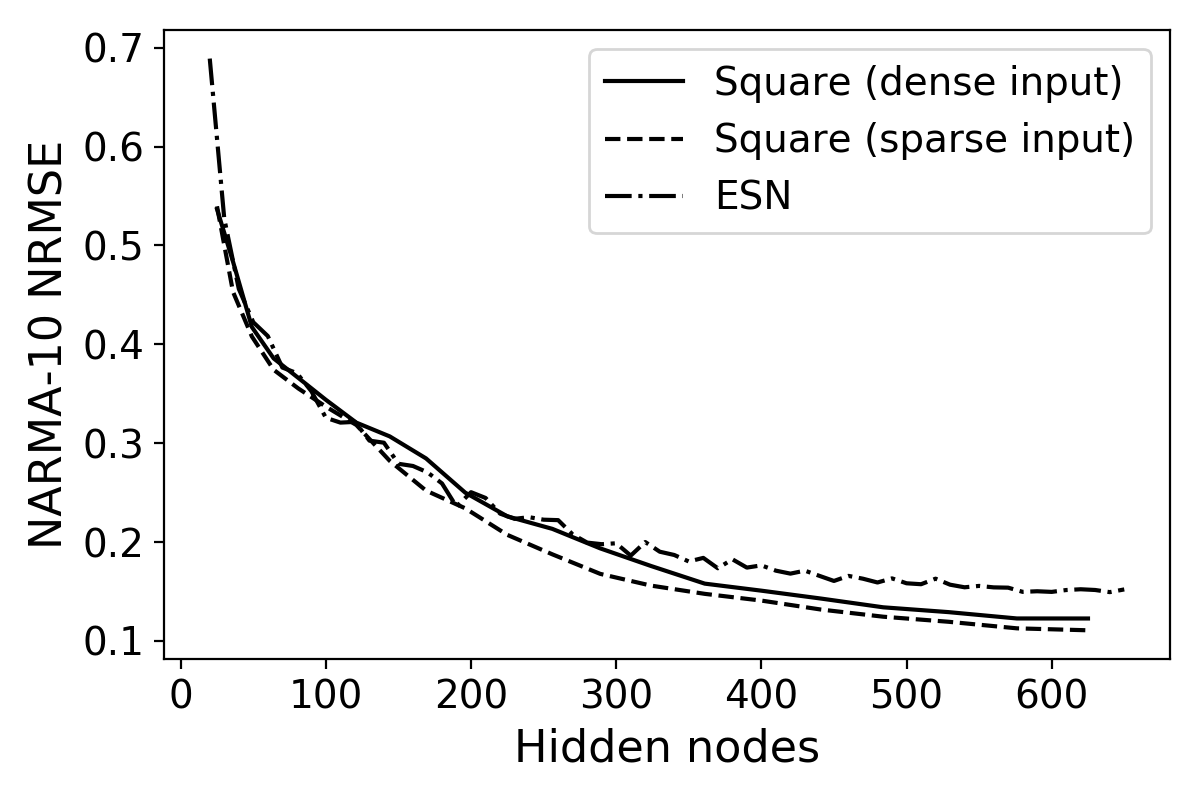
\includegraphics[width=3.5in]{figures/rt-performance-big.png}
  \caption{
    NRMSE of square lattice reservoirs with global, fixed input schemes compared
to standard ESNs. With the sparse input scheme only 50\% of the hidden nodes see
the input.
  }
  \label{fig:rt-performance-big}
\end{figure}

Thus, twice we have found directed edges to improve reservoir performance
significantly, once in random geometric graph reservoirs in Section
\ref{sec:restore}, and now again in lattices. Despite this, lattice reservoirs
still perform slightly worse than ESN.

In the project preceding this thesis, it was found that a global input scheme,
i.e. an input scheme where every input weight is set to 1 and then scaled, works
with ESNs given appropriate scaling \cite{aven_exploring_2019}. This simple
input scheme is relevant to physical RC, given physical substrates in which
every node is forced to see the same input. Results from using this input scheme
with square grids are shown in Figure \ref{fig:rt-performance-big}.

It is abundantly clear that the global input scheme works well with the square
lattice. In fact, it scales even better with reservoir size than the regular
ESNs used in our experiments. Additionally, we have also included error rates
for a square grid with a sparser input scheme in which only 50\% of the hidden
nodes see the input. These networks marginally improve even further upon the
performance of square lattices.

% (TODO): t!
\begin{table}[t]
  \centering
  \begin{center}
    \caption{
      Simplicity of the weighting scheme of square grids. Square grid reservoirs
contain a single unique magnitude for input and reservoir weights. Displayed
values are given as an average across 20 experiment runs (std. dev.).
    }
    \label{tab:sq-global-input}
    \begin{tabular}{c c c c c}
      \hline
      \thead{Reservoir type} & \thead{Hidden \\ nodes} & \thead{Unique \\ input weights} & \thead{Unique \\ reservoir weights} & \thead{NARMA-10 \\ NRMSE} \\
      \hline
      \rule{0pt}{2.5ex}Square grid & 100 & 1 & 1 & 0.346 (0.019) \\
      Square grid & 225 & 1 & 1 & 0.245 (0.022) \\
      Square grid & 400 & 1 & 1 & 0.168 (0.009) \\
      \rule{0pt}{3ex}ESN & 100 & 100 & 997 (26) & 0.388 (0.019) \\
      ESN & 225 & 225 & 5098 (74) & 0.282 (0.019) \\
      ESN & 400 & 400 & 16070 (113) & 0.215 (0.021)\rule[-1ex]{0pt}{0pt} \\
      \hline
    \end{tabular}
  \end{center}
\end{table}

Table \ref{tab:sq-global-input} shows the simplicity of the square grids used in
Figure \ref{fig:rt-performance-big}. The input of the entire reservoir is
decided by a single scalar. Furthermore, there is still only a single unique
magnitude used for reservoir weights in $\mathbf{W}^{res}$, which is determined
by the spacing of nodes.

Simple cyclic reservoirs (SCR) use topology in a similar manner to use a
deterministic weighting scheme \cite{rodan_minimum_2011}. Units in SCRs are
organized in a cycle, with a single unique weight magnitude. All input
connections have the same absolute weight value, but the sign is determined by
means of an unbiased coin. The intention with SCR is to remove stochasticity in
reservoir generation. With square lattices a similar strategy is
employed. However, we do not use a stochastic scheme of generating signed input
values, but instead generate the flow of information in this manner. This leaves
an opportunity to study the structures that are generated, allowing us to peer
into the apparent black box of the ESN, as we shall see in Section
\ref{sec:shrink-grow}.

% (TODO): t!
\begin{figure*}[t]
  \centering
  \begin{subfigure}{.49\textwidth}
    \centering
    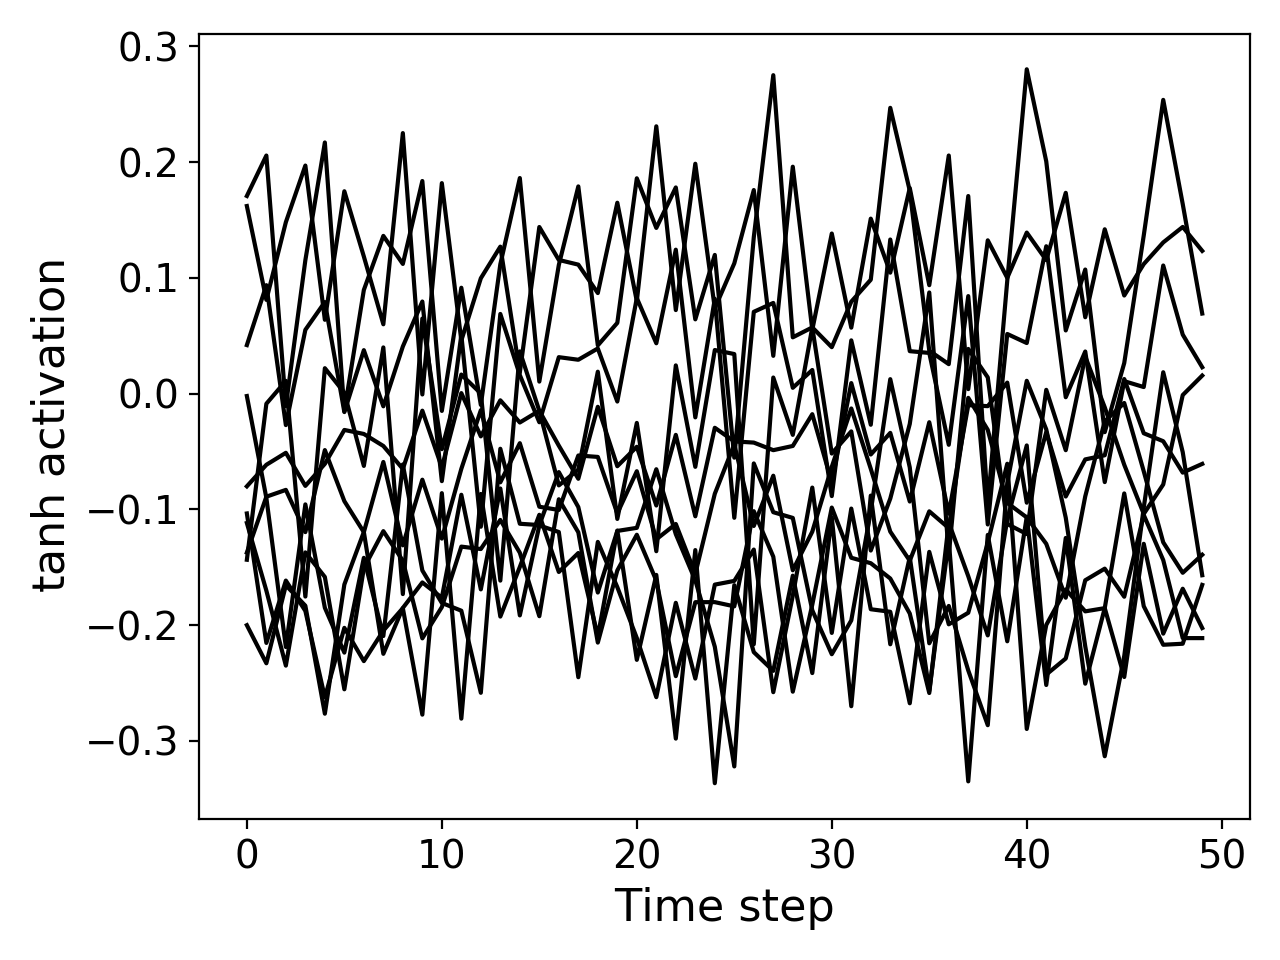
\includegraphics[width=1.0\linewidth]{figures/esn-activations.png}
    \caption{}
    \label{fig:activations-a}
  \end{subfigure}
  \begin{subfigure}{.49\textwidth}
    \centering
    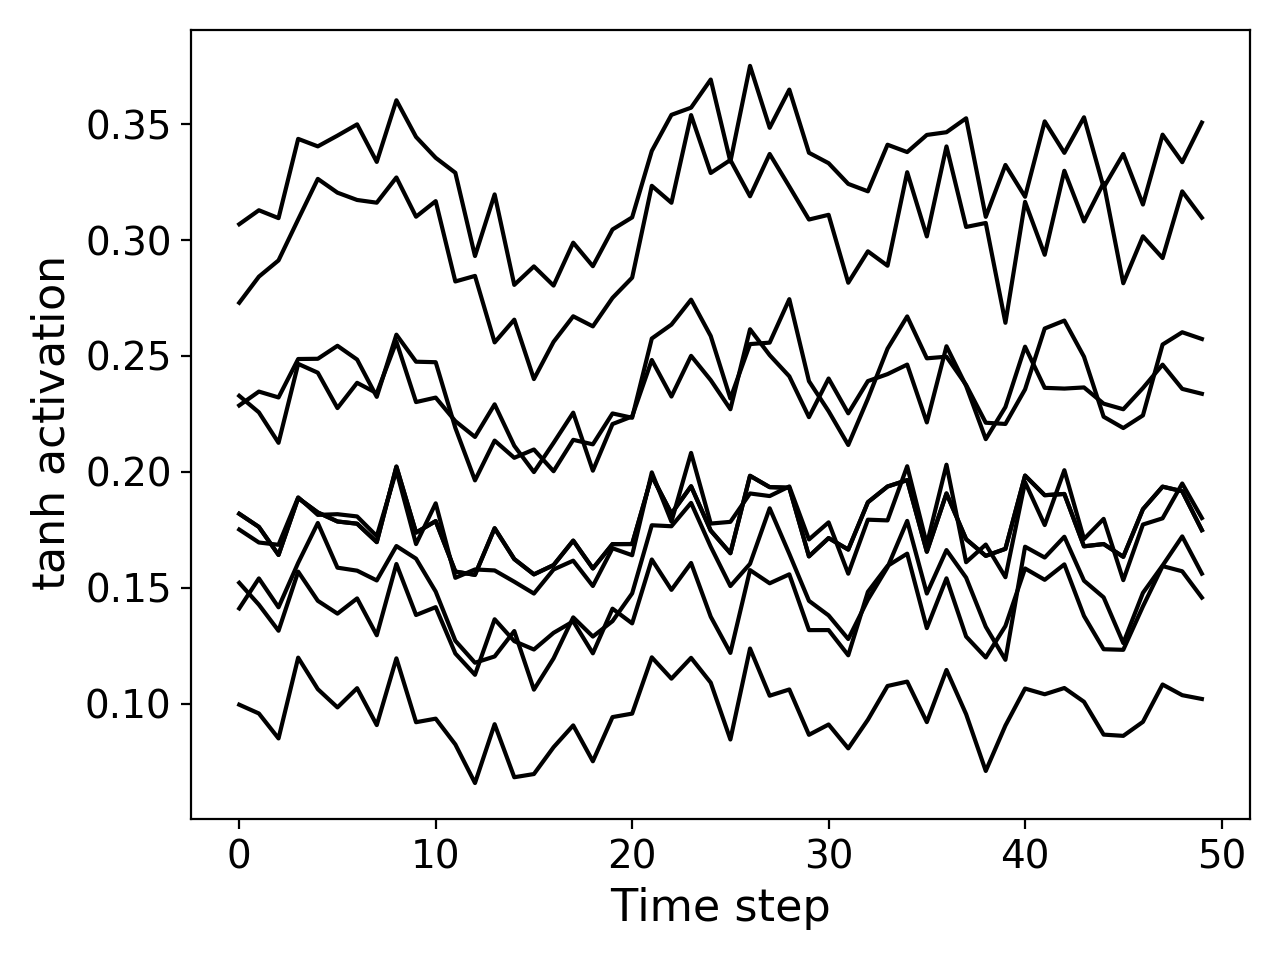
\includegraphics[width=1.0\linewidth]{figures/sq-activations.png}
    \caption{}
    \label{fig:activations-b}
  \end{subfigure}
  \caption{
    Evolution of internal node activations for ESN (a) and square lattice with
global input (b). Reservoirs contain $N = 144$ nodes, but only a subset of 10 is
shown to avoid clutter.
  }
  \label{fig:activations}
\end{figure*}

The evolution of internal node activations proves to be of interest. Figure
\ref{fig:activations} depicts an example run, comparing the standard ESN to
square grids with a fixed, global input scheme. It is clearly visible that nodes
in Figure \ref{fig:activations-b} receive the same input, while uniform
distribution of the ESN in \ref{fig:activations-a} seems more sporadic due to
its uniform input distribution in the interval [-0.5, 0.5].

Note also that the activations of nodes in a square lattice reservoir are
strictly positive, as the NARMA input sequence is strictly positive. This may
warrant a change of activation to other sigmoid functions, as half of $tanh$
remains unused, but has not been investigated further.

In summary, our experimental results demonstrate the potential of designing
reservoirs in a non-stochastic manner. By introducing directed edges to
spatially constrained lattice reservoirs, we have stumbled upon reservoirs that
perform exceptionally well on the NARMA-10 benchmark. These results suggest
that, in a physical RC context, physical substrates will show degraded
performance unless there is a directed flow of information. Additionally, we
propose directed lattice reservoirs as a means to explore this impact of
information flow deeper.

\textcolor{red}{
  Is it worth it to present performance comparisons? The square lattice has a
single scalar input (i.e. no matrix), and a very sparse reservoir matrix. This
might turn out to be quite a lot faster than ESN in practice, but might be
irrelevant.
}

\section{Nonlinear Dynamics in Square Grids}

\subsection{Synopsis}

In this section we look at the potential diversity of nonlinear operations in
square lattice reservoirs. Although the NARMA-10 presents a task of nonlinear
operation, we herein conduct experiments to determine the kernel quality and
generalization capabilities of the square lattice reservoirs, and run benchmarks
with the Mackey-Glass benchmark to generate a mildly chaotic attractor ($\taub =
17$).

\subsection{Results and Discussion}

% (TODO): t!
\begin{figure*}[t]
  \centering
  \begin{subfigure}{.49\textwidth}
    \centering
    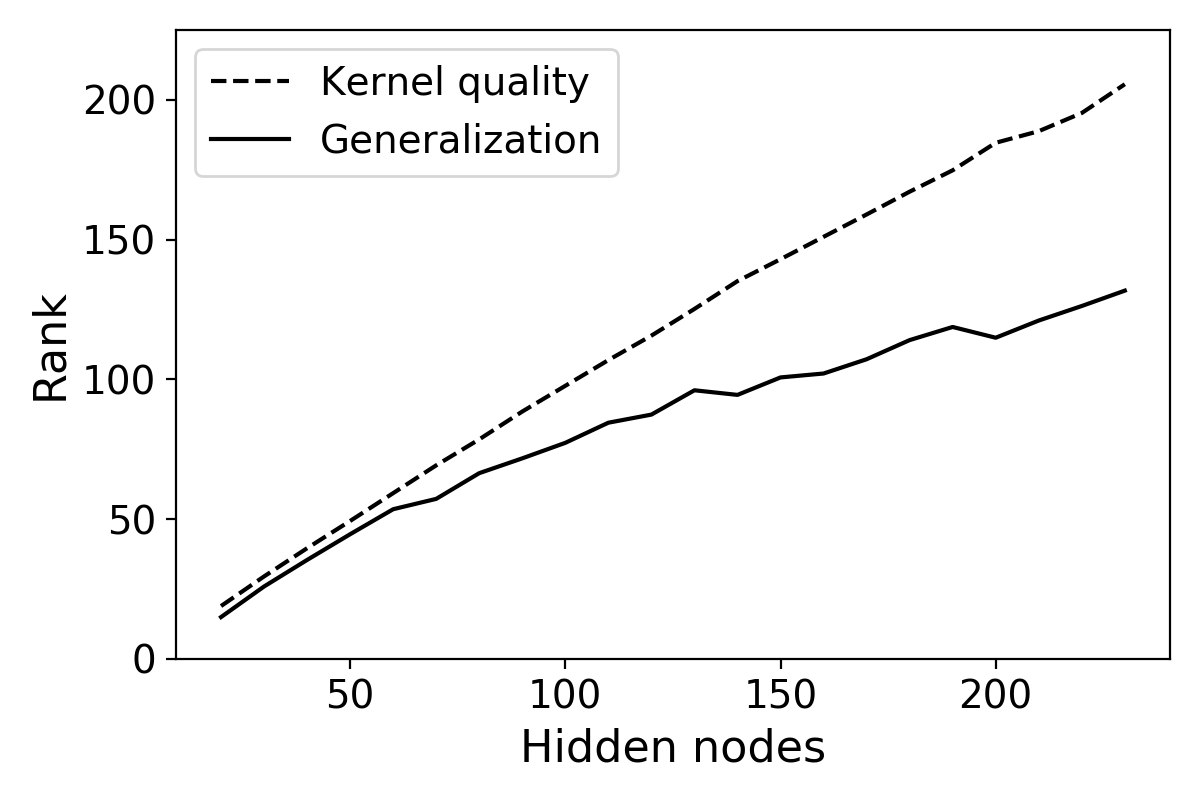
\includegraphics[width=1.0\linewidth]{figures/esn-rank.png}
    \caption{}
    \label{fig:rank-a}
  \end{subfigure}
  \begin{subfigure}{.49\textwidth}
    \centering
    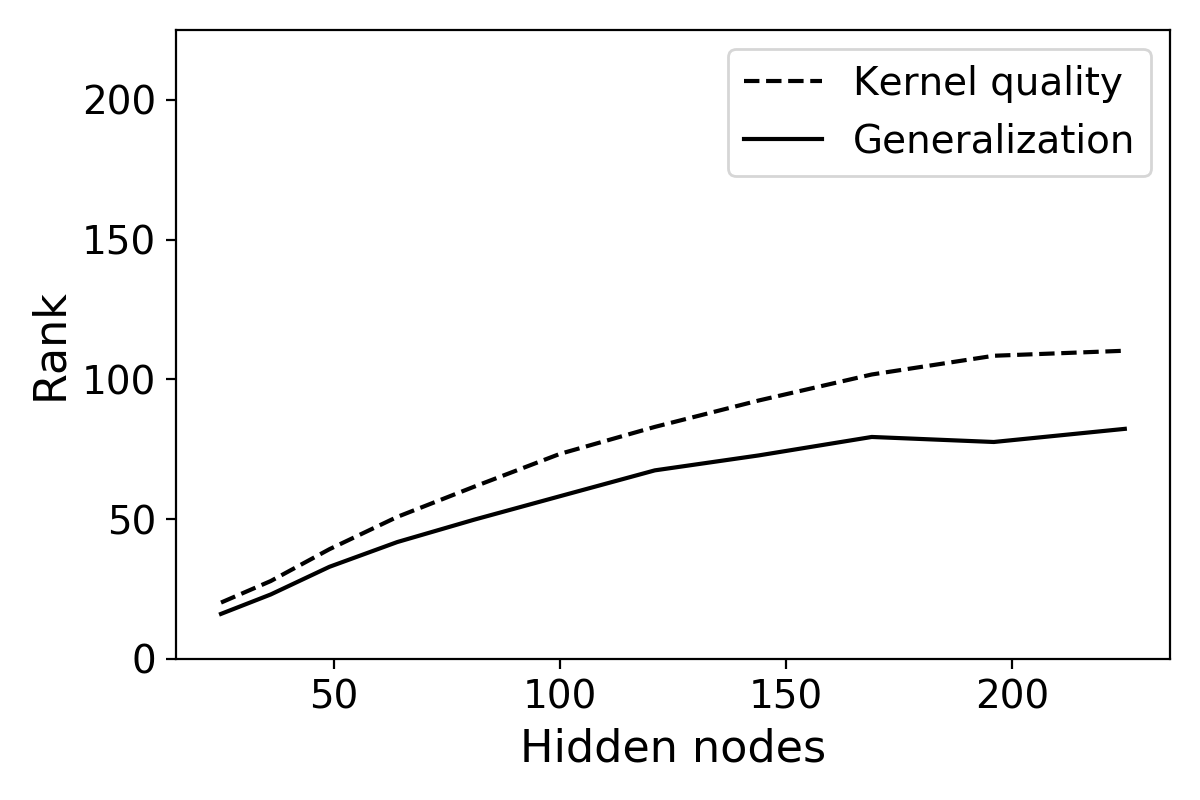
\includegraphics[width=1.0\linewidth]{figures/sq-rank.png}
    \caption{}
    \label{fig:rank-b}
  \end{subfigure}
  \caption{
    Kernel quality and generalization capability as a function of reservoir size
for ESN (a) and square lattice reservoirs (b).
  }
  \label{fig:rank}
\end{figure*}

Consider Figure \ref{fig:rank}, comparing the kernel quality of the default ESN
to square lattice reservoirs. The parameters of the reservoirs remain the same
as in Section \ref{sec:lat-dir-edge}, except a scaling of the ESN spectral
radius to 0.7, as to avoid complete saturation of the respective ranks. We
discover that square lattice reservoirs attain lower kernel
qualities. Additionally the difference between kernel quality and generalization
is also higher for ESN. This difference is often used as a metric of reservoir
quality, as a high kernel quality and low generalization rank is desirable.

If we examine kernel quality (KQ) and generalization rank (G) as a behavior
space $KQ:G$, sweeping parameter spaces will reveal the flexibility of reservoir
types. For all reservoirs, $KQ < N$ and $G < N$, given reservoir size $N$. It is
known that the standard, fully-connected ESN may be tuned to have almost any
$KQ:G$, while lattice reservoirs cover a smaller area of the $KQ:G$ behavior
space, as they are unable to achieve a high $KQ$
\cite{mcquillan_role_2019}. This conclusion is reproduced in Figure
\ref{fig:rank}.

In Section \ref{ssec:topology-and-spatial-networks}, we noted a discrepancy
between performance predicted by kernel quality and benchmarks used by Rodan and
Tiňo in their work on ring topologies. Ring topologies cover a smaller area of
the $KQ:G$ behavior space than fully-connected ESNs. Nonetheless, cyclic
reservoirs with regular jumps (CRJ) consistently outperform ESNs across multiple
benchmarks \cite{rodan_simple_2012}. We see a similar outcome in our experiments
with square lattices, where reservoirs perform comparably on the benchmark, but
exhibit a lower kernel quality. This strengthens a conclusion that
deterministically constructed reservoirs can perform well, given appropriate
tasks.

% (TODO): t!
\begin{figure}[t]
  \centering
  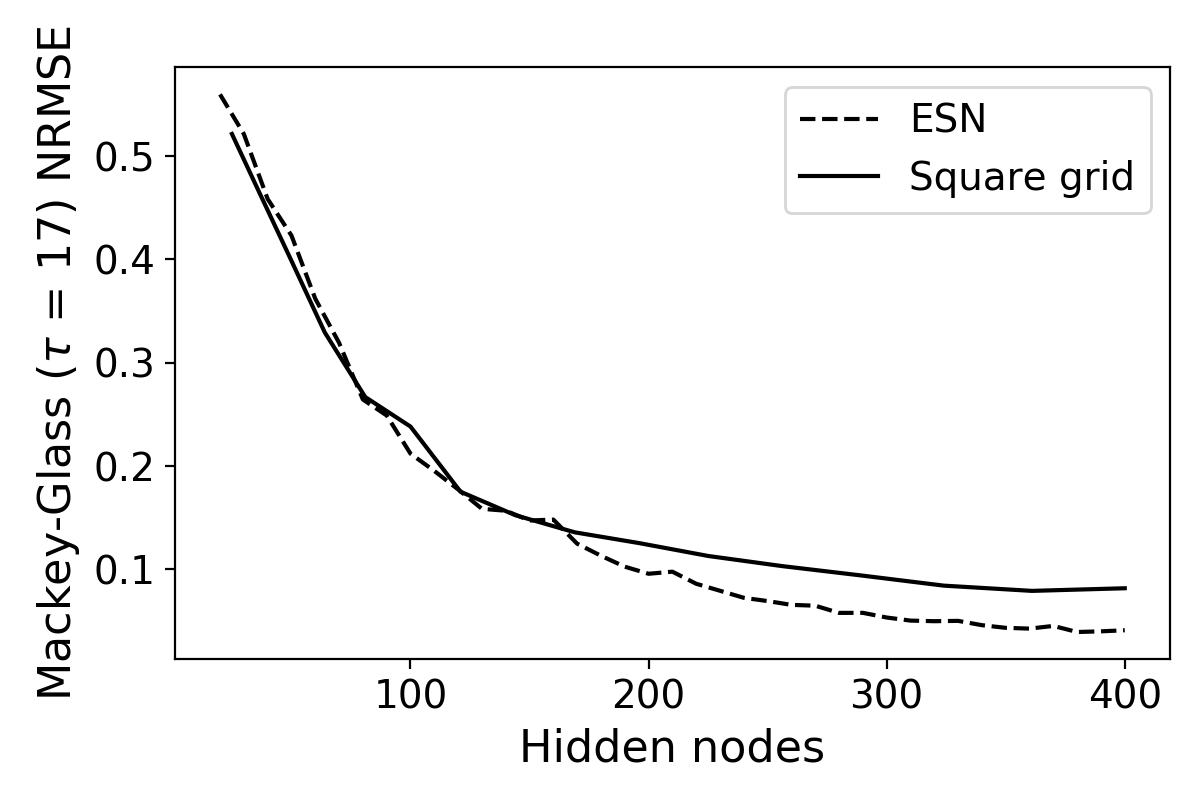
\includegraphics[width=3.5in]{figures/mg17.png}
  \caption{
    NRMSE as a function of reservoir size. Note that this benchmark is the
Mackey-Glass chaotic attractor with $\tau = 17$.
  }
  \label{fig:mg17}
\end{figure}

Figure \ref{fig:mg17} shows NRMSE achieved for square lattice reservoirs on the
Mackey-Glass delay differential equation with mild chaos, $\tau = 17$. Again,
see a comparable performance, although in this case the ESN model scales
slightly better. We would like to stress that previous work commonly compares
reservoirs up to a size of $N = 200$, in which case Figure
\ref{fig:rt-performance-big} and Figure \ref{fig:mg17} show ESN and square
lattice reservoirs to almost perform equally. Thus, from these benchmarks we may
gather that there is potential in lattice reservoirs as simulation models.

\section{Shrinking and Growing Square Grids}
\label{sec:shrink-grow}

\subsection{Synopsis}

\subsection{Results and Discussion}

\textcolor{blue}{
  ``Reservoir computing: Reducing network size and improving
predictionstability'', as well as another paper in mailbox is about simplifying
networks (other is about Shanon information). Maybe useful to talk discuss these
as introduction.
}

\begin{figure}
  \centering
  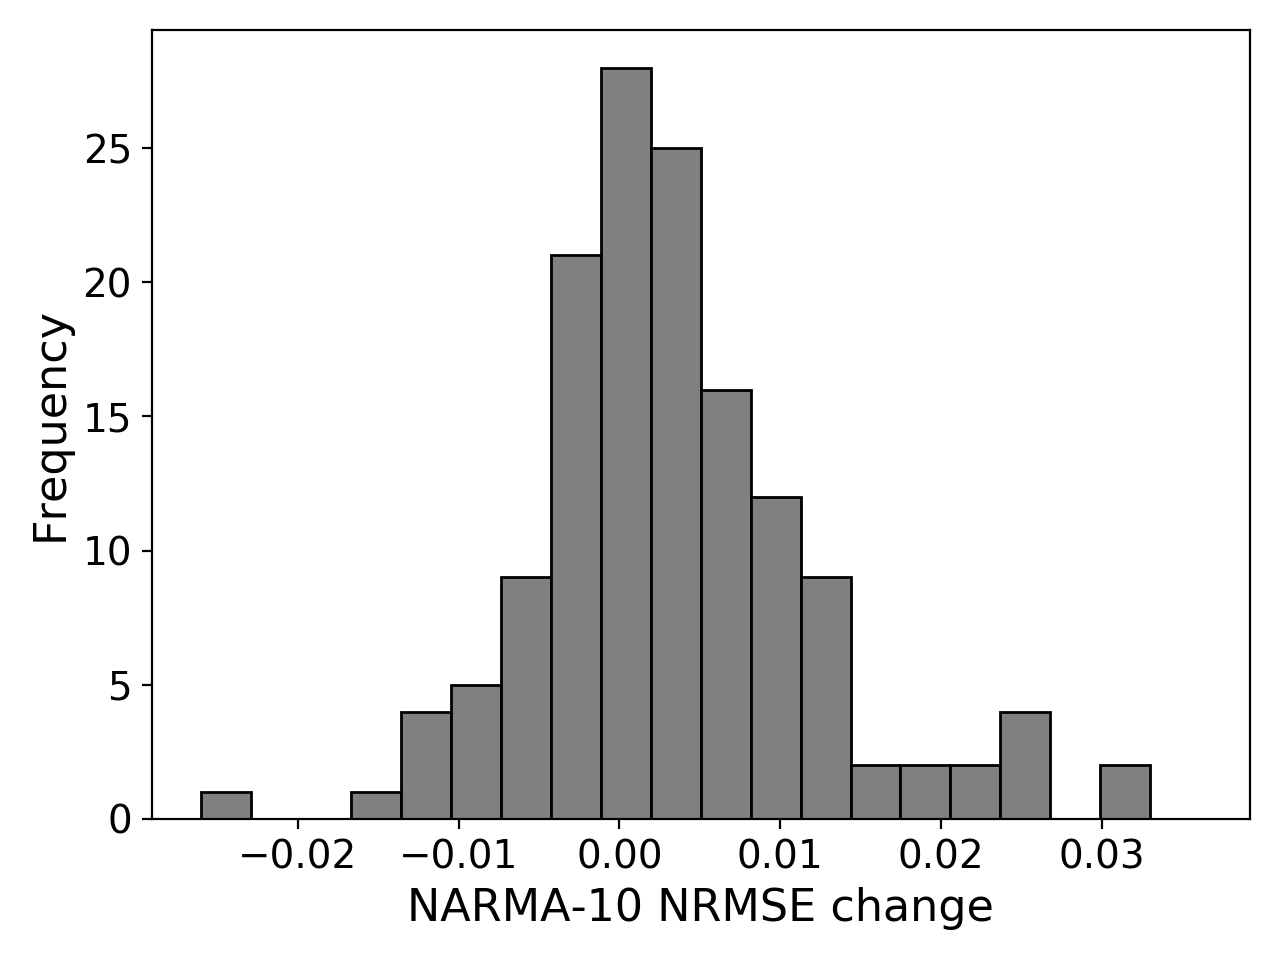
\includegraphics[width=3.5in]{figures/removal-hist.png}
  \caption{
    \textcolor{red}{
      Impact on NARMA-10 NRMSE when removing nodes from a 12x12 square grid
reservoir. No nodes are absolutely essential, while some removals actually
improve overall performance.
    }
  }
  \label{fig:rt-removal-hist}
\end{figure}

\begin{figure}
  \centering
  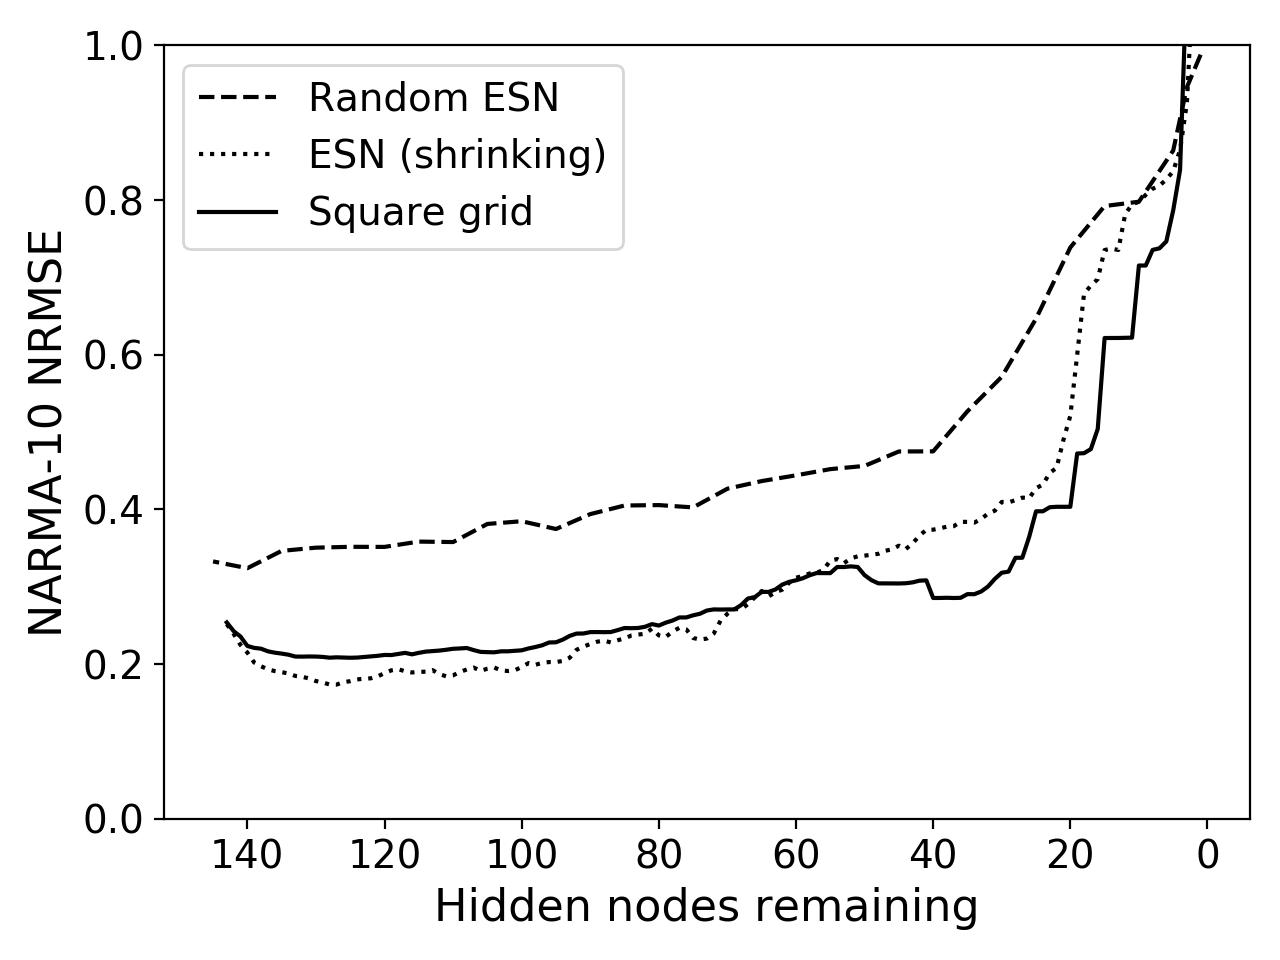
\includegraphics[width=3.5in]{figures/shrink-performance.png}
  \caption{
    \textcolor{red}{
      No caption yet.
    }
  }
  \label{fig:sq-shrink-performance}
\end{figure}

% (TODO): t!
\begin{figure*}[t]
  \centering
  \begin{subfigure}{.40\textwidth}
    \centering
    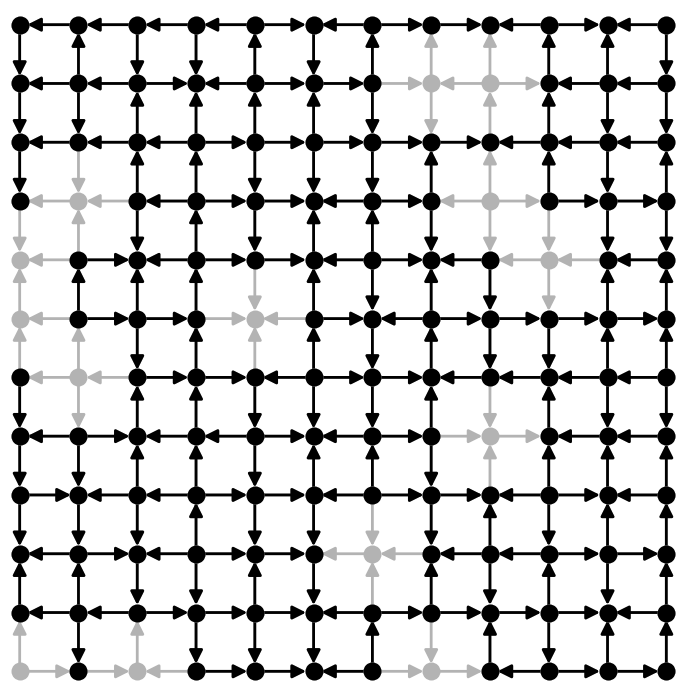
\includegraphics[width=1.0\linewidth]{figures/sq-grid-130.png}
    \caption{}
    \label{fig:sq-grid-130}
  \end{subfigure}
  \begin{subfigure}{.40\textwidth}
    \centering
    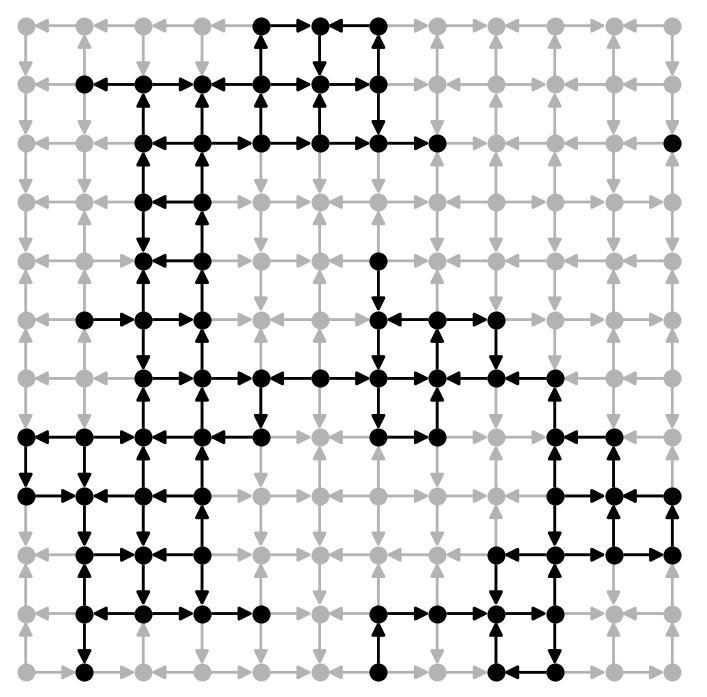
\includegraphics[width=1.0\linewidth]{figures/sq-grid-70.png}
    \caption{}
    \label{fig:sq-grid-70}
  \end{subfigure}
  \vskip\baselineskip

  \begin{subfigure}{.40\textwidth}
    \centering
    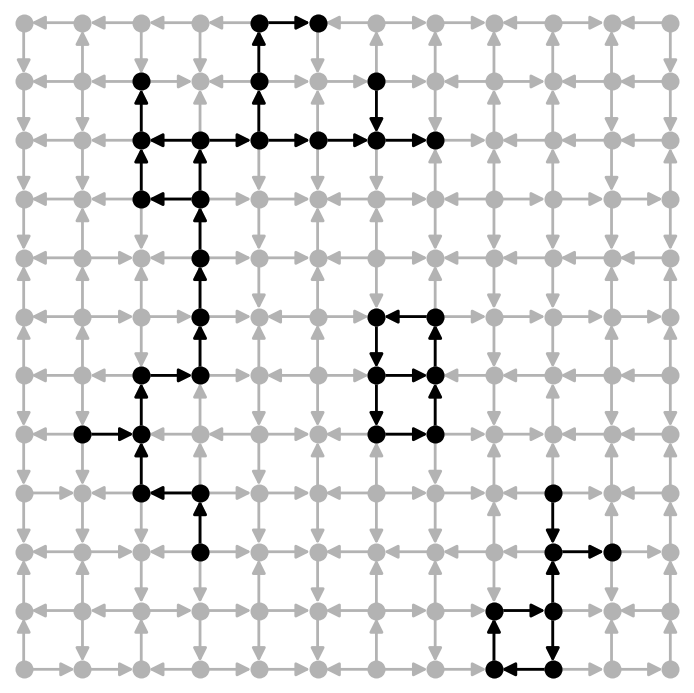
\includegraphics[width=1.0\linewidth]{figures/sq-grid-35.png}
    \caption{}
    \label{fig:sq-grid-35}
  \end{subfigure}
  \begin{subfigure}{.40\textwidth}
    \centering
    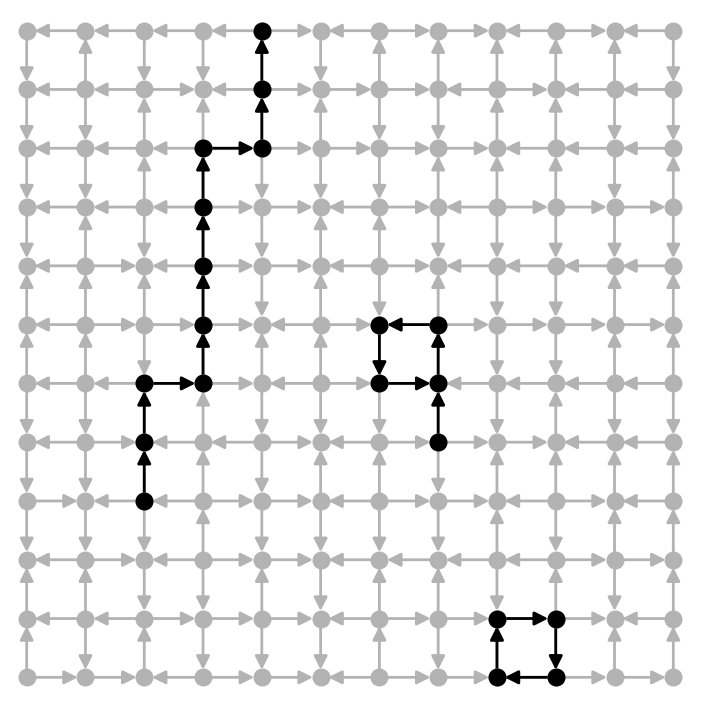
\includegraphics[width=1.0\linewidth]{figures/sq-grid-20.png}
    \caption{\textcolor{red}{Should have NRMSE and nodes left here.}}
    \label{fig:sq-grid-20}
  \end{subfigure}
  \caption{
    \textcolor{red}{
      Progression when incrementally removing nodes from a 12x12 square grid.
    }
  }
  \label{fig:sq-grid}
\end{figure*}

\textcolor{red}{
  Add the example when we have removed nodes from ESN? The one that is just
impossible to make sense of. This is common knowledge however, we could probably
just mention that.
}

\textcolor{red}{
  We need to stress that this is just one example, there is no variance here,
which is a bit of a weakness in the argument.
}

\begin{figure}
  \centering
  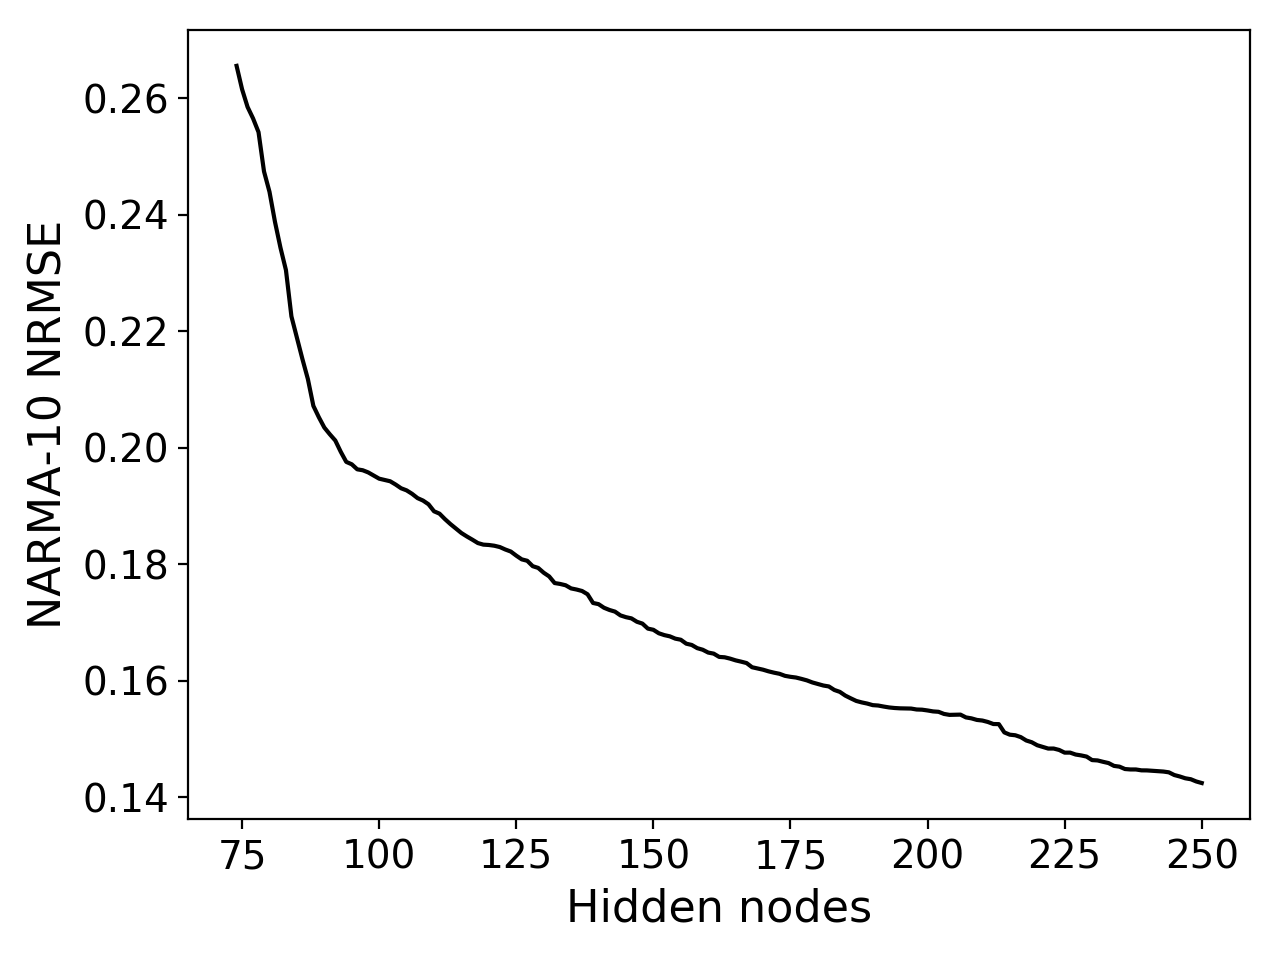
\includegraphics[width=3.5in]{figures/grow-performance.png}
  \caption{
    \textcolor{red}{
      No caption yet.
    }
  }
  \label{fig:sq-grow-performance}
\end{figure}

% (TODO): t!
\begin{figure*}[t]
  \centering
  \begin{subfigure}{1.0\textwidth}
    \centering
    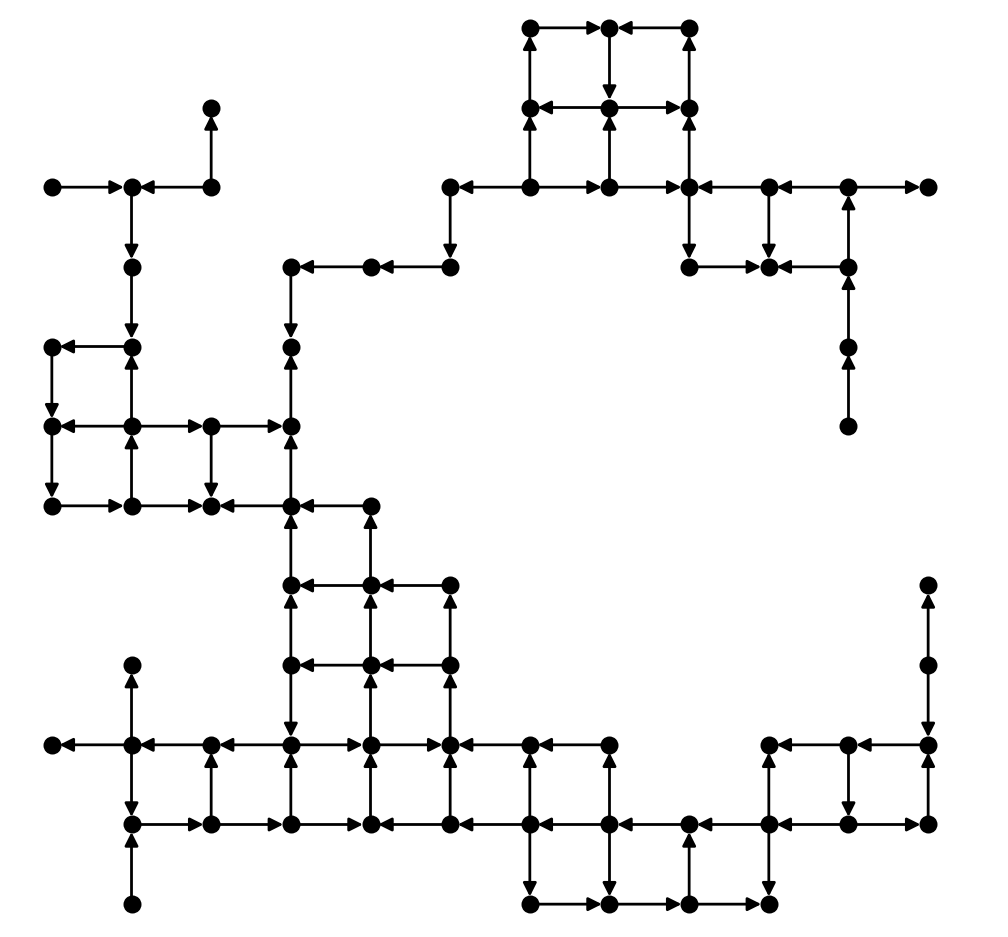
\includegraphics[width=0.5\linewidth]{figures/sq-grid-grow-74.png}
    \caption{}
    \label{fig:sq-grid-grow-74}
  \end{subfigure}
  \begin{subfigure}{.49\textwidth}
    \centering
    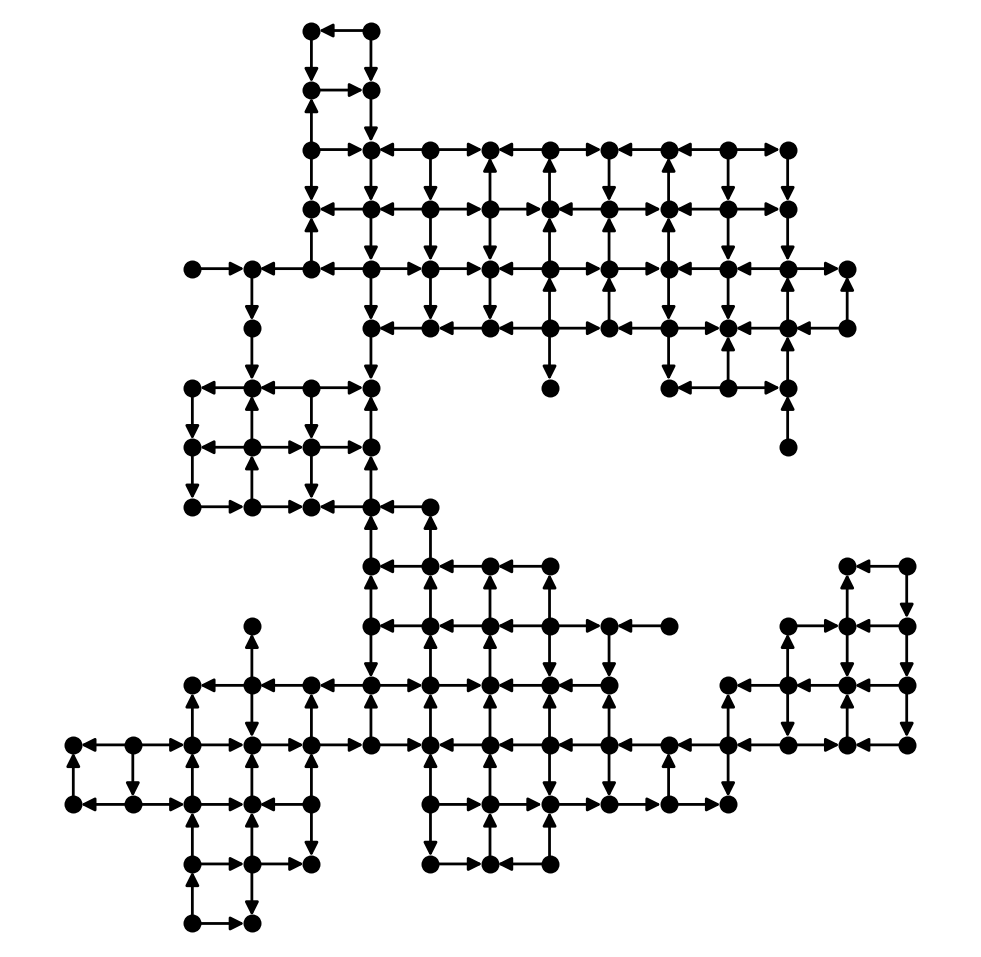
\includegraphics[width=1.0\linewidth]{figures/sq-grid-grow-124.png}
    \caption{}
    \label{fig:sq-grid-grow-124}
  \end{subfigure}
  \begin{subfigure}{.49\textwidth}
    \centering
    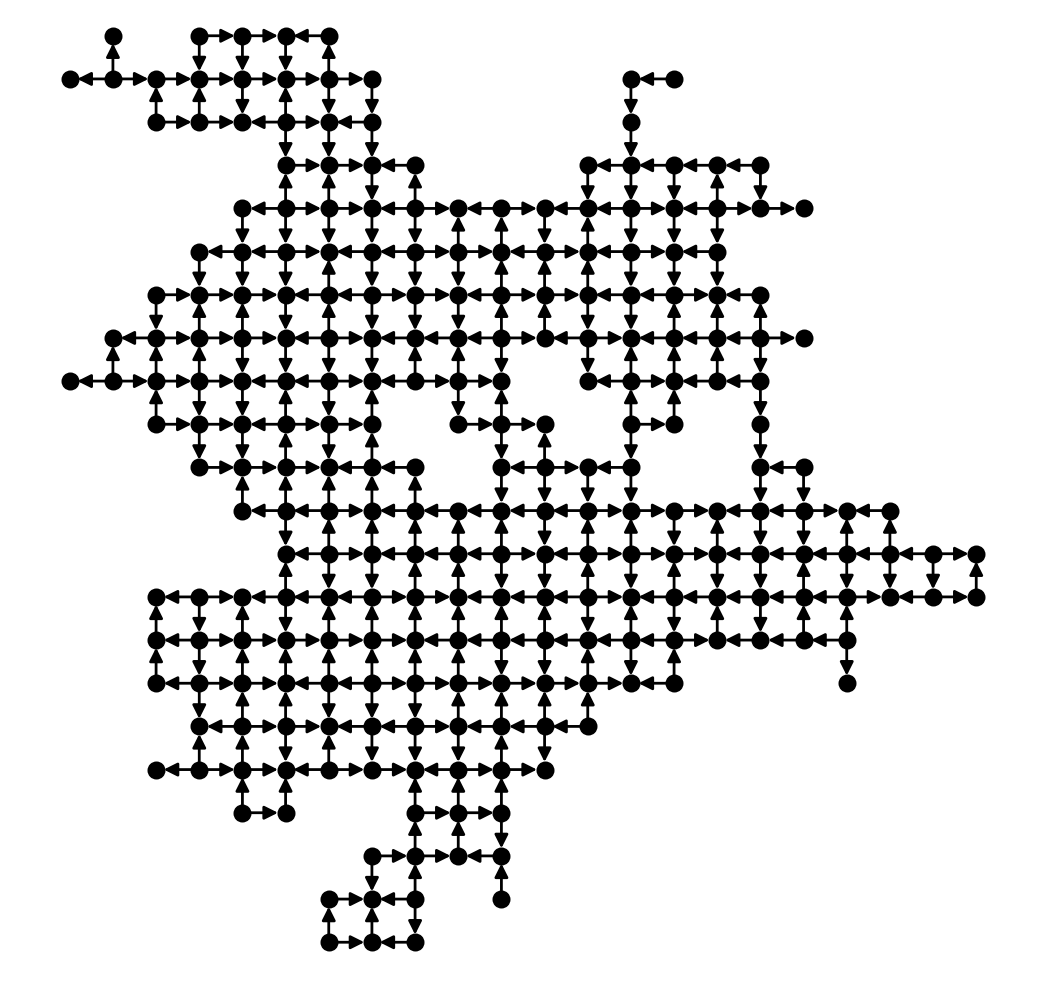
\includegraphics[width=1.0\linewidth]{figures/sq-grid-grow-250.png}
    \caption{\textcolor{red}{Should have captions for NRMSE and size.}}
    \label{fig:sq-grid-grow-250}
  \end{subfigure}
  \caption{
    \textcolor{red}{
      Caption. We see the initial reservoir from where we start growing in (a),
and progress in (b, c).
    }
  }
  \label{fig:sq-grid-grow}
\end{figure*}

\textcolor{red}{
  We repeat the experiment, but this time \textit{adding} nodes along the
frontier, as we can exhaust every possibility for every iteration without that
much trouble. Harder to see what is happening now.
}

\section{Restoring Bidirectional Edges}

\subsection{Synopsis}

\subsection{Results and Discussion}

\begin{figure}
  \centering
  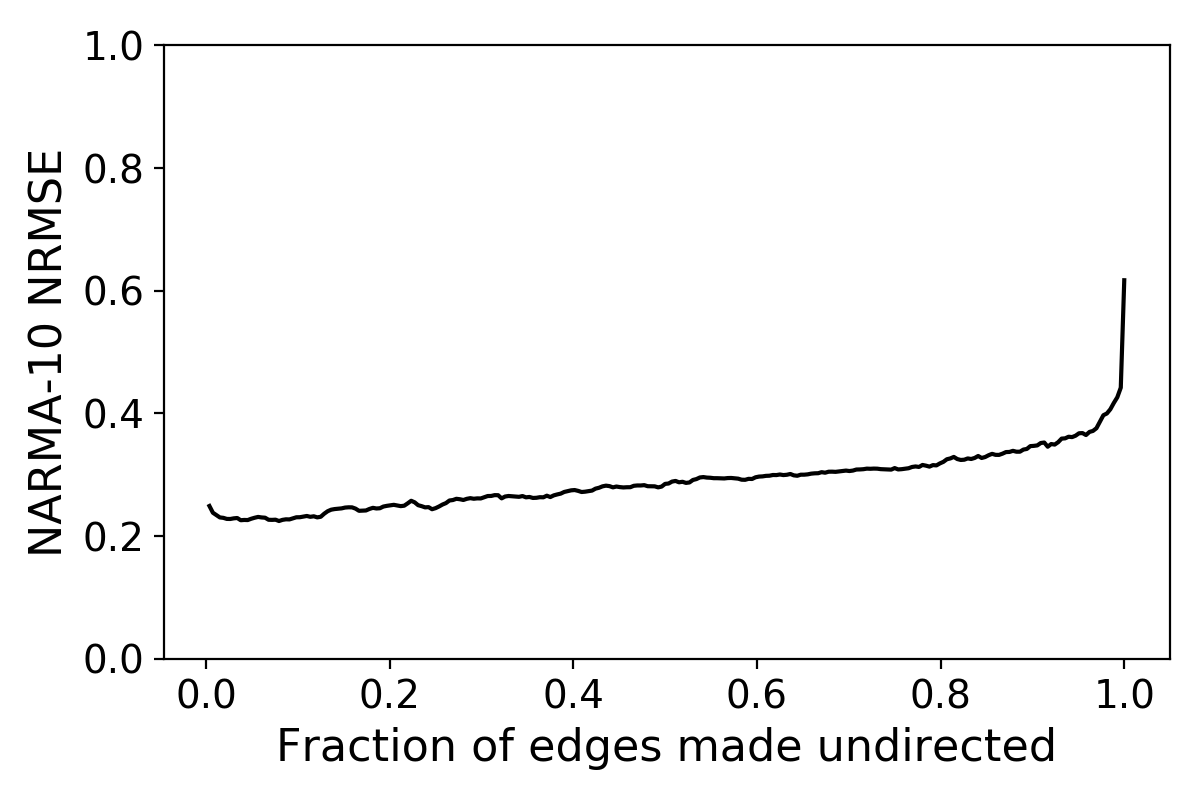
\includegraphics[width=3.5in]{figures/undir-performance.png}
  \caption{
    \textcolor{red}{
      No caption yet. 12x12 square grid.
    }
  }
  \label{fig:undirection-performance}
\end{figure}

\textcolor{red}{
  Imagine something similar to that of Figure \ref{fig:dir-lattice}, where now
only a fraction of the edges are directed again. However, we cannot directly
compare this to that of a cross section of that plot, as we have changed our
input scheme to be global, instead of the uniform distribution that was used
before.
}

\section{Conclusions}

\textcolor{red}{
  Remember that we are not necessarily concerned with finding really good square
grids, but rather that they work at all, since we are concerned with spatial
constraints.
}

\textcolor{red}{
  We find square grids to slightly outperform ESNs on NARMA, and about as good
on MG17.
}

\textcolor{red}{
  We find directedness to be important, and \textit{sufficient}. We find a type
of ESN that is fairly deterministic like CRJ, but has some freedom in
structure. This is useful for exploring ESNs.
}

\textcolor{red}{
  We underline a discrepancy between KQ and actual performance that is already
seen with CRJ. This is quite interesting.
}

\textcolor{red}{
  By analyzing removal of nodes, we find that there seems to be a ``core'' stem
for solving the NARMA task. And ``augmenting'' nodes around. This might be
telling about what happens in ESNs also, but due to randomness.
}

\textcolor{red}{
  We find that removing nodes and evaluating can be good to remove noisy nodes.
}


%%% Local Variables:
%%% mode: latex
%%% TeX-master: "../thesis"
%%% End:
